% Copyright 2004 by Till Tantau <tantau@users.sourceforge.net>.
%
% In principle, this file can be redistributed and/or modified under
% the terms of the GNU Public License, version 2.
%
% However, this file is supposed to be a template to be modified
% for your own needs. For this reason, if you use this file as a
% template and not specifically distribute it as part of a another
% package/program, I grant the extra permission to freely copy and
% modify this file as you see fit and even to delete this copyright
% notice. 

\documentclass[utf8]{beamer}

\usepackage[utf8]{inputenc}
\usepackage[croatian]{babel}

% There are many different themes available for Beamer. A comprehensive
% list with examples is given here:
% http://deic.uab.es/~iblanes/beamer_gallery/index_by_theme.html
% You can uncomment the themes below if you would like to use a different
% one:
%\usetheme{AnnArbor}
%\usetheme{Antibes}
%\usetheme{Bergen}
%\usetheme{Berkeley}
%\usetheme{Berlin}
%\usetheme{Boadilla}
%\usetheme{boxes}
%\usetheme{CambridgeUS}
%\usetheme{Copenhagen}
%\usetheme{Darmstadt}
%\usetheme{default}
%\usetheme{Frankfurt}
%\usetheme{Goettingen}
%\usetheme{Hannover}
%\usetheme{Ilmenau}
%\usetheme{JuanLesPins}
%\usetheme{Luebeck}
\usetheme{Madrid}
%\usetheme{Malmoe}
%\usetheme{Marburg}
%\usetheme{Montpellier}
%\usetheme{PaloAlto}
%\usetheme{Pittsburgh}
%\usetheme{Rochester}
%\usetheme{Singapore}
%\usetheme{Szeged}
%\usetheme{Warsaw}

\title[Implementacija RTS igre]{Implementacija jezgrenih funkcionalnosti RTS-igre}

% A subtitle is optional and this may be deleted
\subtitle{Završni rad br. 5173}

\author{Leon Luttenberger}

\institute[FER]
{
    Fakultet elektrotehnike i računarstva\\
    Sveučilište u Zagrebu
}

\date{5.~srpnja 2017.}

\subject{}
% This is only inserted into the PDF information catalog. Can be left
% out. 

% If you have a file called "university-logo-filename.xxx", where xxx
% is a graphic format that can be processed by latex or pdflatex,
% resp., then you can add a logo as follows:

% \pgfdeclareimage[height=0.5cm]{university-logo}{university-logo-filename}
% \logo{\pgfuseimage{university-logo}}

% Delete this, if you do not want the table of contents to pop up at
% the beginning of each subsection:
\AtBeginSubsection[]
{
    \begin{frame}<beamer>{Sadržaj}
        \tableofcontents[currentsection,currentsubsection]
    \end{frame}
}

\begin{document}

\begin{frame}
    \titlepage
\end{frame}

\begin{frame}{Sadržaj}
    \tableofcontents
    % You might wish to add the option [pausesections]
\end{frame}

\section{Uvod}

\subsection{Opis zadatka}

\begin{frame}{Opis zadatka}{}
    \begin{itemize}
        \item {
            Proučiti i implementirati osnovne podsustave prisutne u RTS-igrama
        }
        \item {
            Implementirati prototip jedne konkretne igre
        }
        \item {
            Implementaciju ostvariti u programskom jeziku Java
        }
    \end{itemize}
\end{frame}

\subsection{RTS}

\begin{frame}{RTS}
    \begin{itemize}
        \item {
            \textit{Real-Time Strategy}
        }
        \item {   
            Tipična RTS-igra sadrži sljedeće elemente.
            \begin{itemize}
                \item Mapa
                \item Skupljanje resursa
                \item Izgradnja zgrada
                \item Jedinice
            \end{itemize}
        }
    \end{itemize}
\end{frame}

\section{Podsustavi}

\subsection{Kretanje jedinica}
% Uređivanje mapa
% dodavanje funkcionalnosti

\begin{frame}{Pronalazak najkraćeg puta}
    \begin{figure}[h] 
        \centering
        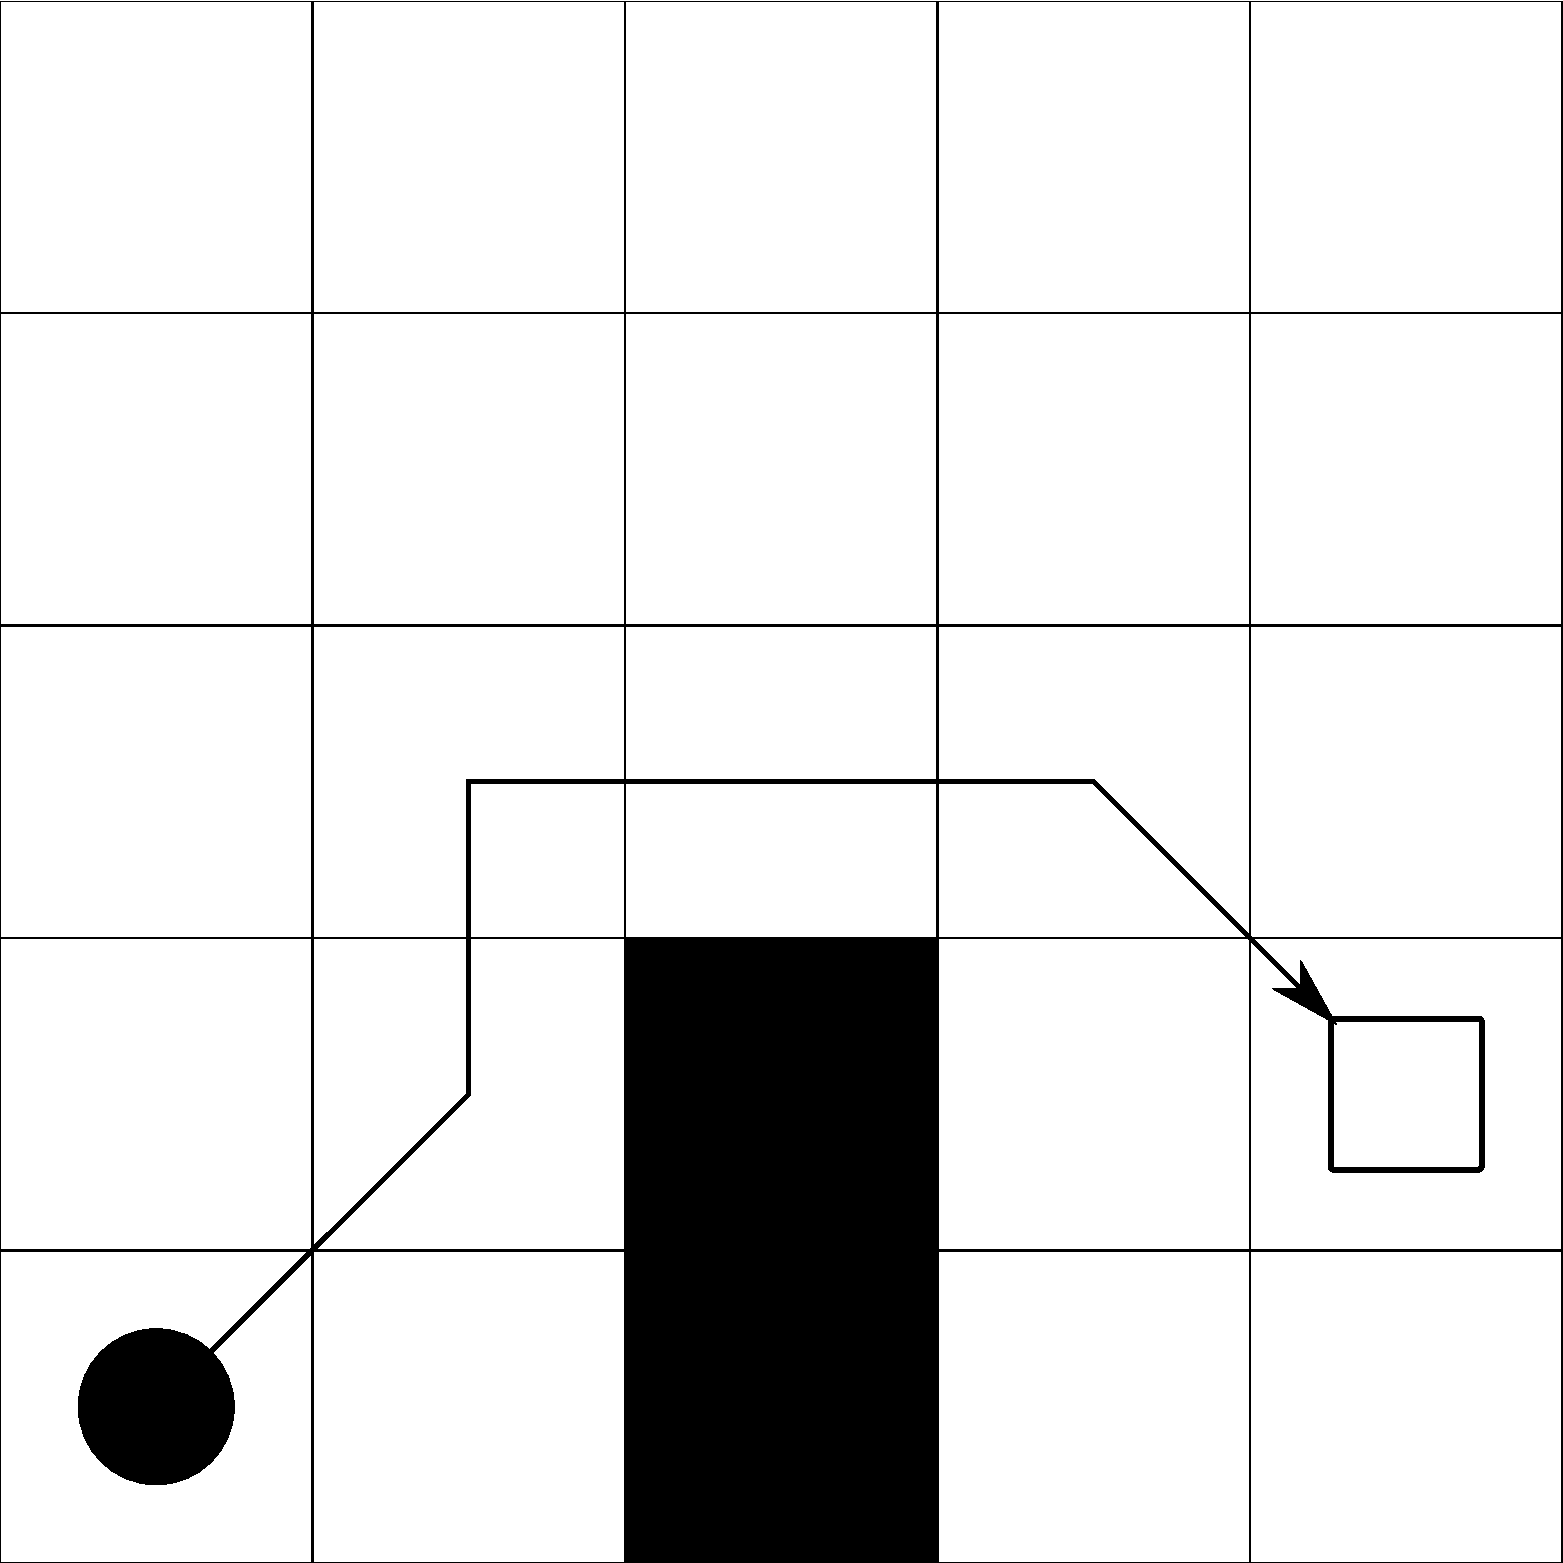
\includegraphics[height=4cm]{images/basicGrid.pdf}
    \end{figure} 
\end{frame}

\begin{frame}{Algoritam A*}
    \begin{itemize}
        \item Algoritam za usmjerenu pretragu
        \item Ubacuje stanja u prioritetni red prema vrijednosti \(f(s) = g(s) + h(s)\)
    \end{itemize}
\end{frame}

\begin{frame}{Svojstva heuristike}
    \begin{block}{Optimičnost}<1->
        Heuristika ne smije precijeniti trošak puta, odnosno:
        \(\forall s \in S, h(s) \leq h^*(s)\).
    \end{block}
  
    \begin{block}{Konzistentnost}<2->
        Procjena udaljenosti trenutnog stanja ne smije biti veća od procjene udaljenosti susjednog stanja i njene udaljenosti od trenutnog stanja, odnosno:
        \(h(s) \leq c(s, a) + h(s')\).
    \end{block}

    \only<3>{
        \begin{figure}[h]
            \centering
            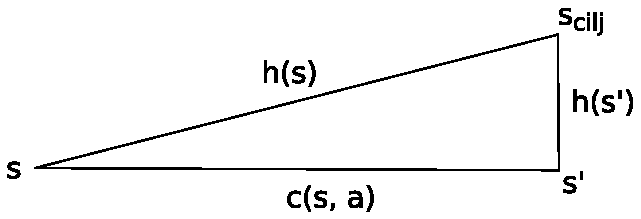
\includegraphics[height=2.5cm]{images/triangleInequality.pdf}
        \end{figure} 
    }

    \begin{block}{Objaviještenost}<4->
        Veće vrijednosti heuristika nam daju bolju informaciju o udaljenosti.
    \end{block}
\end{frame}

\begin{frame}{Problemi sa algoritmom A*}
    \begin{itemize}
        \item Preskup za primjenu u realnom vremenu
        \item Ne može se prilagoditi na promjene
    \end{itemize}
\end{frame}

\begin{frame}{Ponovljeni A*}
    \only<1>{
        \begin{itemize}
            \item Ograničimo pretragu na lokalni prostor stanja
            \item Prilikom dolaska na najbolje pronađeno stanje, pretraga se ponovo pokrene
            \item Pretraga se ponovo izvrši i ako na putu naiđemo na promjenu
        \end{itemize}
    }

    \only<2>{
        \begin{figure}[h]
            \centering
            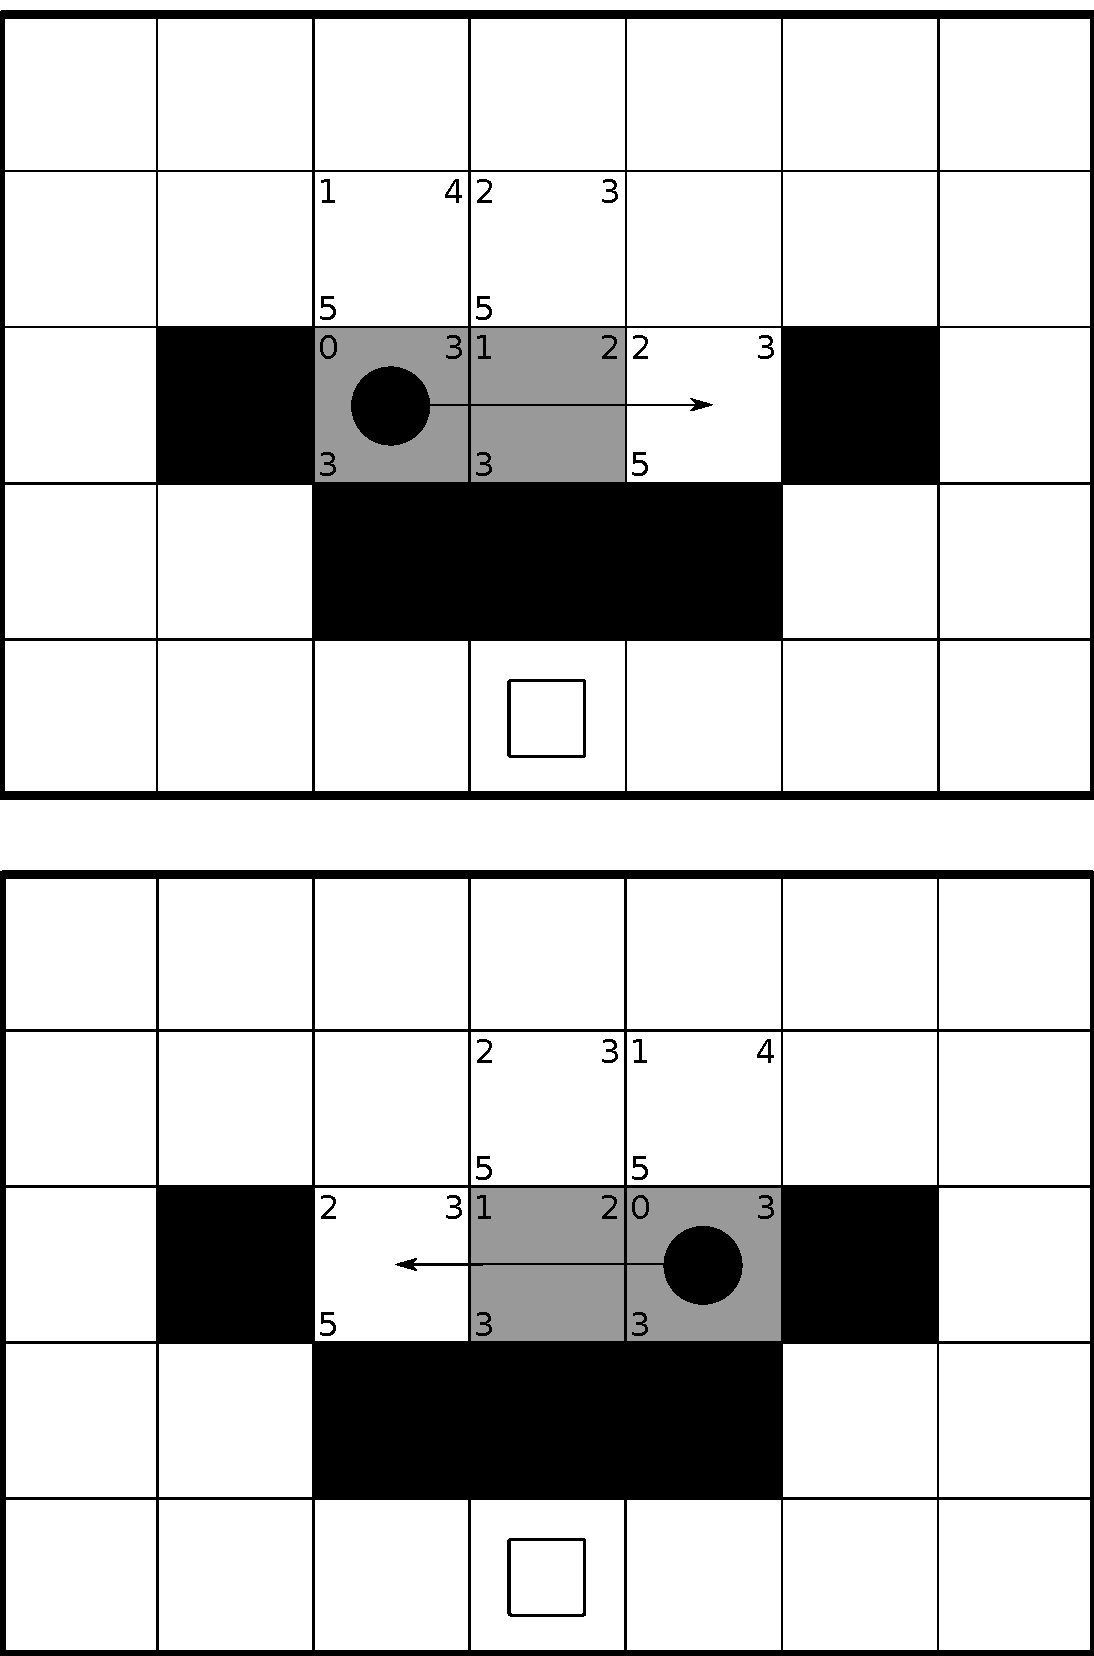
\includegraphics[height=7.5cm]{images/repeatedAStarCycle.pdf}
        \end{figure} 
    }
\end{frame}

\begin{frame}{Adaptivni A* u stvarnom vremenu}
    \only<1> {
        \begin{itemize}
            \item \(\forall s \in S, h(s_{start}) \leq g(s) + h(s)\)

            \item {
                Uvrštavanjem uvjeta konzistentnosti u navedenu relaciju dobivamo:
                \(
                \begin{aligned}
                & \forall s \in S, f(\overline{s}) \leq g(s) + h(s)\\
                & \forall s \in S, h(s) \geq f(\overline{s}) - g(s)
                \end{aligned}
                \)
            }

            \item { 
                Za svako posjećeno stanje moguće je napraviti sljedeću korekciju:
                
                \[h(s) = f(\overline{s}) - g(s)\]
            }
        \end{itemize}
    }

    \only<2> {
        \begin{figure}[h]
            \centering
            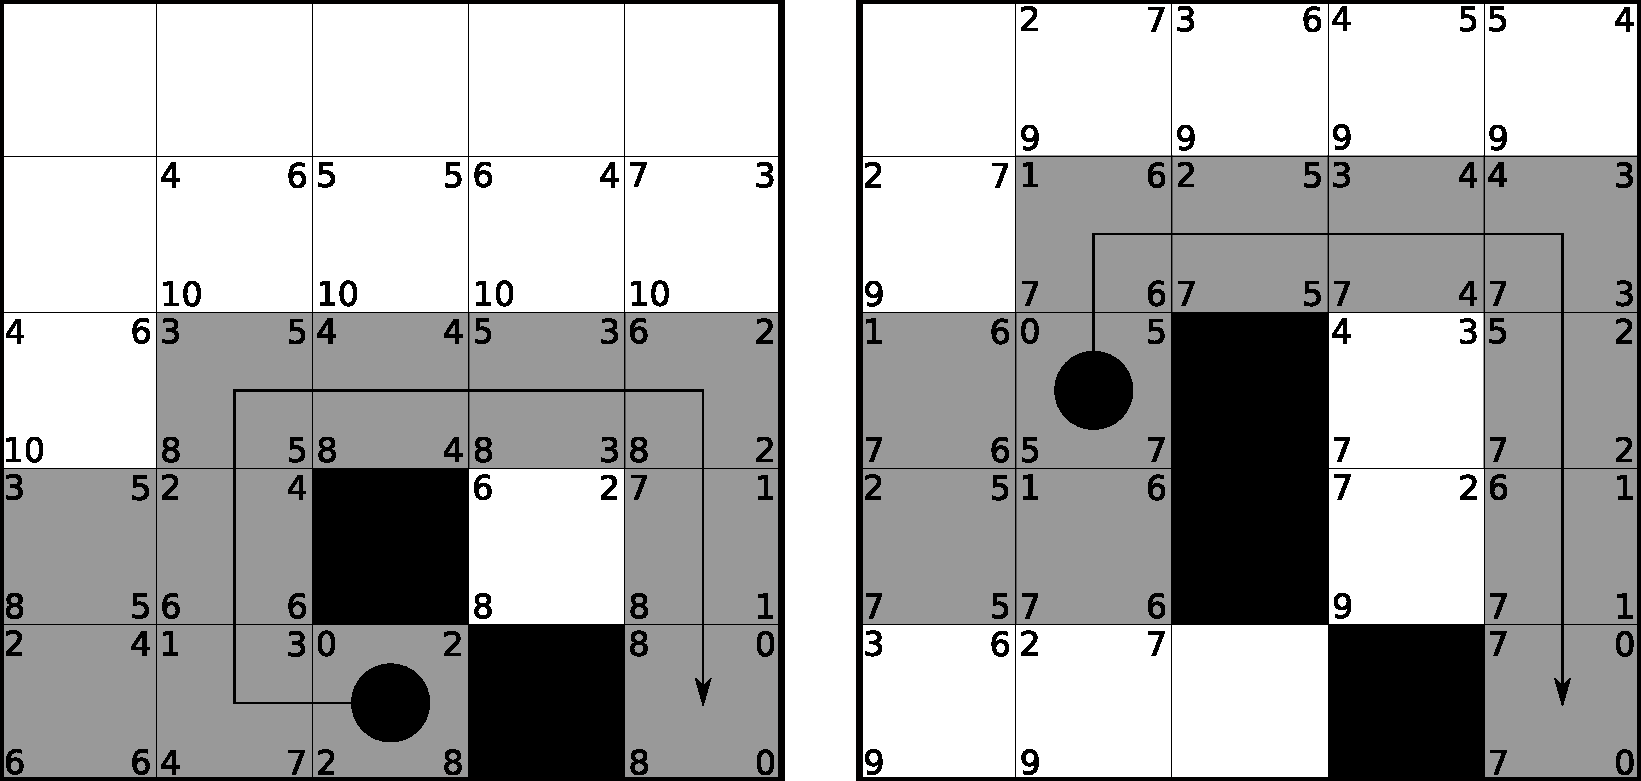
\includegraphics[height=5cm]{images/rtaastar.pdf}
        \end{figure}
    }
\end{frame}

\begin{frame}{Grupiranje: algoritam \textit{Boids}}
    Tri osnovna pravila:
    \begin{figure}[h]
        \centering
        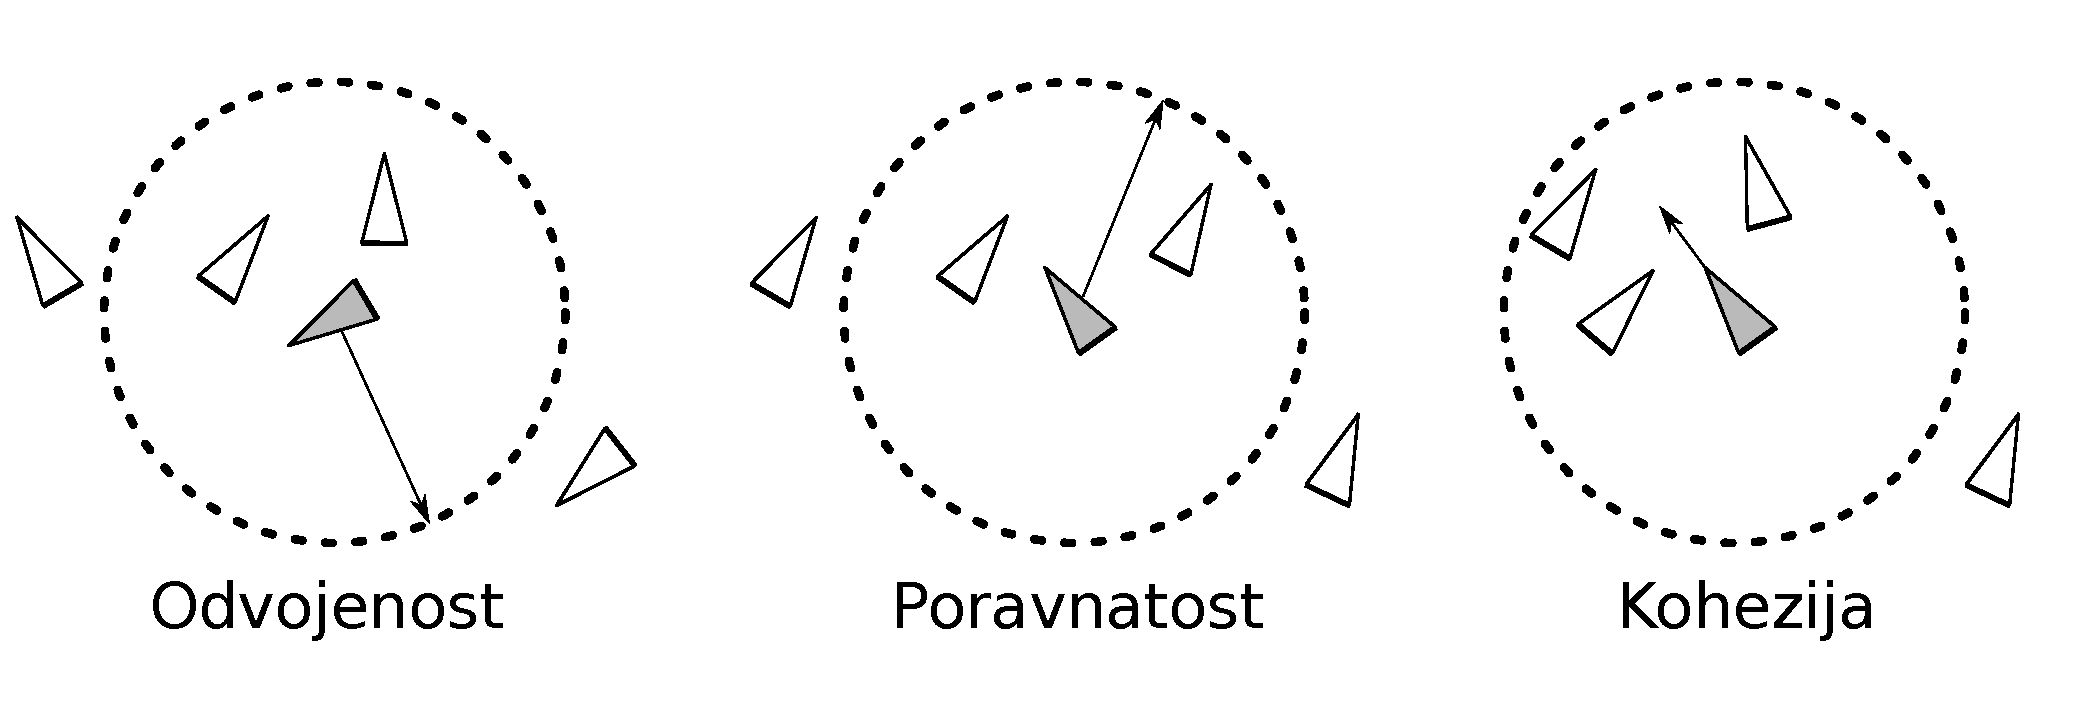
\includegraphics[width=1.0\linewidth]{images/boids.pdf}
    \end{figure}
\end{frame}

\section{Demonstracija}

% Placing a * after \section means it will not show in the
% outline or table of contents.
\section*{Summary}

\begin{frame}{Summary}
  \begin{itemize}
  \item
    The \alert{first main message} of your talk in one or two lines.
  \item
    The \alert{second main message} of your talk in one or two lines.
  \item
    Perhaps a \alert{third message}, but not more than that.
  \end{itemize}
  
  \begin{itemize}
  \item
    Outlook
    \begin{itemize}
    \item
      Something you haven't solved.
    \item
      Something else you haven't solved.
    \end{itemize}
  \end{itemize}
\end{frame}

\end{document}